\documentclass[usenames,dvipsnames,aspectratio=169]{beamer}
\usepackage{../common/prg}

\usepackage{array}
\newcolumntype{C}[1]{>{\centering\let\newline\\\arraybackslash\hspace{0pt}}m{#1}}

\title[9. előadás]{Programozás}
\subtitle{(GKxB\_INTM114)}

\begin{document}

%1
\begin{frame}[plain]
  \titlepage
  \logoalul
\end{frame}

%2
\section{Különleges mátrixok}
\subsection{Motiváló feladat -- városok közötti távolság}
\begin{frame}
  Feladat:
  \begin{itemize}
    \item két város nevének beolvasása,
    \item városok közötti távolság megjelenítése.
    \item Kilépés azonos városok megadása esetén.
  \end{itemize}
  \vfill
  Megoldás:
  \begin{itemize}
    \item városok nevét vektorban tároljuk
    \item a városok közötti távolságokat pedig mátrixban, és
    \item a városok vektorbeli indexével indexeljük a mátrixot is
  \end{itemize}
\end{frame}

%3
\begin{frame}[fragile]
  \begin{block}{Kimenet}
    \begin{verbatim}
Varosok kozotti tavolsag kiszamitasa
Kilepes azonos varosok megadasaval.
Indulo varos: Budapest
Erkezesi varos: Salakszentmotoros
Nem letezo varos!
Gyor
Tavolsag: 121km
Indulo varos: Gyor
Erkezesi varos: Gyor
\end{verbatim}
  \end{block}
\end{frame}

%4
\begin{frame}
  \begin{exampleblock}{\textattachfile{varosok1.cpp}{varosok1.cpp}}
    \footnotesize
    \lstinputlisting[style=cpp,linerange={36-49},numbers=left,firstnumber=36]{varosok1.cpp}
  \end{exampleblock}
\end{frame}

%5
\begin{frame}
  \begin{exampleblock}{\textattachfile{varosok1.cpp}{varosok1.cpp}}
    \scriptsize
    \vspace{-.2cm}
    \lstinputlisting[style=cpp,linerange={5-21},numbers=left,firstnumber=5]{varosok1.cpp}
    \vspace{-.2cm}
  \end{exampleblock}
\end{frame}

%6
\begin{frame}
  \begin{exampleblock}{\textattachfile{varosok1.cpp}{varosok1.cpp}}
    \vspace{-.2cm}
    \lstinputlisting[style=cpp,linerange={23-34},numbers=left,firstnumber=23]{varosok1.cpp}
    \vspace{-.2cm}
  \end{exampleblock}
\end{frame}

%7
\subsection{,,Háromszögmátrixok'': eltérő elemszámú vektorok tömbje}
\begin{frame}
  Észrevétel: a mátrixnak több, mint fele elhagyható! ($m_{i,j}=m_{j,i}, m_{i,i} = 0$)
  \begin{center}
    \small
    \begin{tabular}{r|ccccccc}
                  & \rotatebox{90}{Budapest} & \rotatebox{90}{Győr} & \rotatebox{90}{Szeged} &
                    \rotatebox{90}{Debrecen} & \rotatebox{90}{Veszprém} & \rotatebox{90}{Dunaújváros} &
                    \rotatebox{90}{Eger} \\ \hline
      Budapest    & \kiemelZ{0}  & 121 & 174 & 231 & 115 &  83 & 139 \\
      Győr        & \kiemel{121} & \kiemelZ{0}  & 287 & 377 &  82 & 176 & 285 \\
      Szeged      & \kiemel{174} & \kiemel{287} & \kiemelZ{0}  & 218 & 278 & 161 & 298 \\
      Debrecen    & \kiemel{231} & \kiemel{377} & \kiemel{218} & \kiemelZ{0}  & 368 & 320 & 131 \\
      Veszprém    & \kiemel{115} & \kiemel{82}  & \kiemel{278} & \kiemel{368} & \kiemelZ{0}  & 103 & 275 \\
      Dunaújváros & \kiemel{83}  & \kiemel{176} & \kiemel{161} & \kiemel{320} & \kiemel{103} & \kiemelZ{0}  & 228 \\
      Eger        & \kiemel{139} & \kiemel{285} & \kiemel{298} & \kiemel{131} & \kiemel{275} & \kiemel{228} & \kiemelZ{0} \\
    \end{tabular}
  \end{center}
  Probléma: a mátrixnak minden sora azonos elemszámú\\
  Megoldás: eltérő elemszámú vektorokat címző vektor létrehozása (mutatótömb, alsó háromszögmátrix)
\end{frame}

%8
\begin{frame}
  \begin{exampleblock}{\textattachfile{varosok2.cpp}{varosok2.cpp}}
    \scriptsize
    \vspace{-.2cm}
    \lstinputlisting[style=cpp,linerange={24-39},numbers=left,firstnumber=24]{varosok2.cpp}
    \vspace{-.2cm}
  \end{exampleblock}
\end{frame}

%9
\subsection{,,Háromszögmátrixok'': eltérő elemszámú vektorok egymás után}
\begin{frame}
  Észrevétel: még a vektorokat címző mutatók is megtakaríthatók, ha sorfolytonosan, egyetlen vektorban tároljuk a főátló alatti 
értékeket!
  \begin{center}
    \scriptsize
    \begin{tabular}{r|cccccc}
                  & \rotatebox{90}{Bp. [0]} & \rotatebox{90}{Győr [1]} & \rotatebox{90}{Szeged [2]} &
                    \rotatebox{90}{Debr. [3]} & \rotatebox{90}{Veszp. [4]} & \rotatebox{90}{Duv. [5]}\\ \hline
      Győr [1]        & \kiemelZ{121} & & & & & \\
      Szeged [2]      & \kiemelZ{174} & \kiemelZ{287} & & & & \\
      Debrecen [3]    & \kiemelZ{231} & \kiemelZ{377} & \kiemelZ{218} & & & \\
      Veszprém [4]    & \kiemel{115} & \kiemel{82} & 278 & 368 & & \\
      Dunaújváros [5] & 83 & 176 & 161 & 320 & 103 & \\
      Eger [6]        & 139 & 285 & 298 & 131 & 275 & 228 \\
    \end{tabular}\\
    \vspace{.3cm}
    \begin{tabular}{c|cc|ccc|cccc}
      [0] & [1] & [2] & [3] & [4] & [5] & [6] & [7] & [8] & [9] \\ \hline
      \kiemelZ{121} & \kiemelZ{174} & \kiemelZ{287} & \kiemelZ{231} & \kiemelZ{377} & \kiemelZ{218} & 
        \kiemel{115} & \kiemel{82} & 278 & \dots \\
    \end{tabular}
  \end{center}
  Keresett elem feletti sorokban lévő adatok száma sorról sorra számtani sort alkot \\
  $S_n = \frac{[2a_1 + (n-1)d] \cdot n}{2}$, speciálisan $a_1=1, d=1 \to S_n = \frac{(n+1) \cdot n}{2}$
\end{frame}

%10
\begin{frame}
  \begin{exampleblock}{\textattachfile{varosok3.cpp}{varosok3.cpp}}
    \scriptsize
    \vspace{-.2cm}
    \lstinputlisting[style=cpp,linerange={24-40},numbers=left,firstnumber=24]{varosok3.cpp}
    \vspace{-.2cm}
  \end{exampleblock}
\end{frame}

%11
\subsection{Statikus változók}
\begin{frame}
  Probléma:
  \begin{itemize}
    \item a lokális változók alapértelmezetten \emph{automatikusak} (ld. \hiv{\href{https://en.cppreference.com/w/cpp/keyword/auto}{\texttt{auto}}}, C++11-ig): élettartam a definíció pillanatától a 
blokk elhagyásáig tart
    \item a vektorok és tömbök újrafoglalása időigényes
  \end{itemize}
  \vfill
  Megoldás: \hiv{\href{https://en.cppreference.com/w/cpp/language/storage_duration\#Static_local_variables}{\texttt{static}}} minősítő használata
  \begin{itemize}
    \item élettartam: program indulásától leállásig $\to$ értéküket megőrzik a függvényhívások között
    \item hatókör: változatlan (deklarációtól blokk végéig)
    \item implicit módon inicializált (feltöltés zérus értékű bitekkel)
  \end{itemize}
\end{frame}

%12
\begin{frame}
  \begin{exampleblock}{\textattachfile{varosok4.cpp}{varosok4.cpp}}
    \scriptsize
    \vspace{-.2cm}
    \lstinputlisting[style=cpp,linerange={6-22},numbers=left,firstnumber=6]{varosok4.cpp}
    \vspace{-.2cm}
  \end{exampleblock}
\end{frame}

%13
\subsection{Dinamikus ,,háromszögmátrixok''}
\begin{frame}
  Feladat: 
  \begin{itemize}
    \item hozzuk létre futásidőben a vektort és a háromszögmátrixot!
    \item töltsük fel őket felhasználó által adott értékekkel!
  \end{itemize}
  \begin{exampleblock}{\textattachfile{varosok5.cpp}{varosok5.cpp}}
    \scriptsize
    \vspace{-.2cm}
    \lstinputlisting[style=cpp,linerange={57-68},numbers=left,firstnumber=57]{varosok5.cpp}
    \vspace{-.2cm}
  \end{exampleblock}
\end{frame}

%14
\begin{frame}
  \begin{exampleblock}{\textattachfile{varosok5.cpp}{varosok5.cpp} -- \texttt{main}}
    \footnotesize
    \lstinputlisting[style=cpp,linerange={69-82},numbers=left,firstnumber=69]{varosok5.cpp}
  \end{exampleblock}
\end{frame}

%15
\begin{frame}
  \begin{exampleblock}{\textattachfile{varosok5.cpp}{varosok5.cpp}}
    \lstinputlisting[style=cpp,linerange={5-12},numbers=left,firstnumber=5]{varosok5.cpp}
  \end{exampleblock}
\end{frame}

%16
\begin{frame}
  \begin{exampleblock}{\textattachfile{varosok5.cpp}{varosok5.cpp}}
    \vspace{-.2cm}
    \lstinputlisting[style=cpp,linerange={27-38},numbers=left,firstnumber=27]{varosok5.cpp}
    \vspace{-.2cm}
  \end{exampleblock}
\end{frame}

%17
\begin{frame}
  \begin{exampleblock}{\textattachfile{varosok5.cpp}{varosok5.cpp}}
    \vspace{-.2cm}
    \lstinputlisting[style=cpp,linerange={14-25},numbers=left,firstnumber=14]{varosok5.cpp}
    \vspace{-.2cm}
  \end{exampleblock}
\end{frame}

%18
\begin{frame}
  \begin{exampleblock}{\textattachfile{varosok5.cpp}{varosok5.cpp}}
    \lstinputlisting[style=cpp,linerange={40-48},numbers=left,firstnumber=40]{varosok5.cpp}
  \end{exampleblock}
\end{frame}

%19
\begin{frame}
  \begin{exampleblock}{\textattachfile{varosok5.cpp}{varosok5.cpp}}
    \lstinputlisting[style=cpp,linerange={50-55},numbers=left,firstnumber=50]{varosok5.cpp}
  \end{exampleblock}
\end{frame}

%20
\section{Négyzetes mátrixok: a bűvös négyzet}
\subsection{Tulajdonságok}
\begin{frame}
  \begin{itemize}
    \item Bűvös négyzet: olyan (ált. 1 és $n^2$ közötti) egész számokat tartalmazó négyzetes mátrix, melynek
    \begin{itemize}
      \item minden sorösszege,
      \item minden oszlopösszege,
      \item főátlójában és
      \item mellékátlójában lévő számok összege azonos.
    \end{itemize}
    \item \hiv{\href{http://en.wikipedia.org/wiki/Magic_square}{További érdekességek}}
  \end{itemize}
  \begin{center}
    \tiny
    \begin{tabular}{cc}
      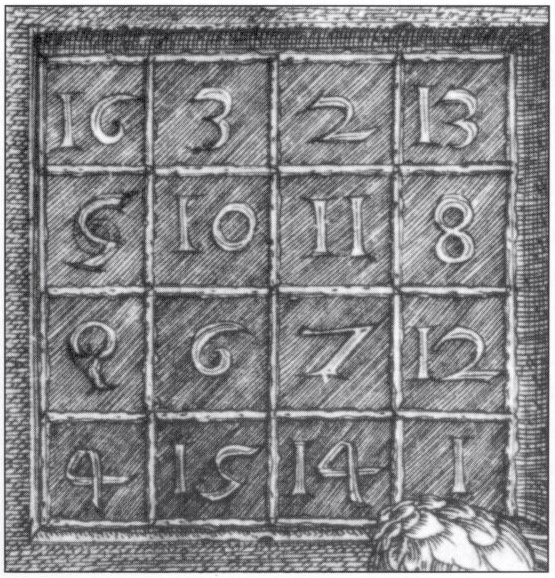
\includegraphics[height=3cm]{melancolia.jpg} & 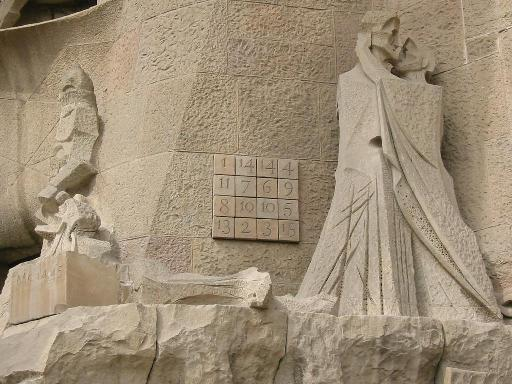
\includegraphics[height=3cm]{sagrada.jpg} \\
      Albrecht Dürer: Melencolia I (részlet) & Sagrada Família, Barcelona\\
    \end{tabular}
  \end{center}
\end{frame}

%21
\subsection{Páratlan rendű bűvös négyzet előállítása}
\begin{frame}
  \scriptsize
 \hiv{\href
 {http://en.wikipedia.org/wiki/Magic_square\#A_method_for_constructing_a_magic_square_of_odd_order}
 {Páratlan rendű bűvös négyzetek konstrukciója}}
  \begin{enumerate}
    \item A mátrix első sorának középső oszlopába írjunk 1-et!
    \item A mátrix minden további elemének értéke legyen eggyel nagyobb a korábbinál (2, 3, \dots,
$n^2$)!
    \item A következő elemet úgy választjuk ki, hogy \kiemel{jobbra és felfelé} lépünk egyet.
    \begin{itemize}
      \scriptsize
      \item Ha a meghatározott elem már korábban ki lett töltve, akkor az utoljára kitöltött elem
\kiemel{alatti} elemmel kell folytatni a műveletet.
      \item Ha az így meghatározott elem kívül esne a mátrixon, akkor a szemközti oldalon lévő első
elemet kell használni (pl. a ,,legfelső feletti'' sor esetén a legalsót).
    \end{itemize}
  \end{enumerate}
  \begin{center}
    \begin{tabular}{|C{.2cm}|C{.2cm}|C{.2cm}|}
      \hline
      \multicolumn{3}{|c|}{1. lépés}\\
      \hline
       & 1 &  \\
      \hline
       &  &  \\
      \hline
       &  &  \\
      \hline
    \end{tabular}
    \begin{tabular}{|C{.2cm}|C{.2cm}|C{.2cm}|}
      \hline
      \multicolumn{3}{|c|}{2. lépés}\\
      \hline
       & 1 &  \\
      \hline
       &  &  \\
      \hline
       &  & 2 \\
      \hline
    \end{tabular}
    \begin{tabular}{|C{.2cm}|C{.2cm}|C{.2cm}|}
      \hline
      \multicolumn{3}{|c|}{3. lépés}\\
      \hline
       & 1 &  \\
      \hline
      3 &  &  \\
      \hline
       &  & 2 \\
      \hline
    \end{tabular}
    \begin{tabular}{|C{.2cm}|C{.2cm}|C{.2cm}|}
      \hline
      \multicolumn{3}{|c|}{4. lépés}\\
      \hline
       & 1 &  \\
      \hline
      3 &  &  \\
      \hline
      4 &  & 2 \\
      \hline
    \end{tabular}
    \begin{tabular}{|C{.2cm}|C{.2cm}|C{.2cm}|}
      \hline
      \multicolumn{3}{|c|}{5. lépés}\\
      \hline
       & 1 &  \\
      \hline
      3 & 5 &  \\
      \hline
      4 &  & 2 \\
      \hline
    \end{tabular}
    \begin{tabular}{|C{.2cm}|C{.2cm}|C{.2cm}|}
      \hline
      \multicolumn{3}{|c|}{6. lépés}\\
      \hline
       & 1 & 6 \\
      \hline
      3 & 5 &  \\
      \hline
      4 &  & 2 \\
      \hline
    \end{tabular}
    \begin{tabular}{|C{.2cm}|C{.2cm}|C{.2cm}|}
      \hline
      \multicolumn{3}{|c|}{7. lépés}\\
      \hline
       & 1 & 6 \\
      \hline
      3 & 5 & 7 \\
      \hline
      4 &  & 2 \\
      \hline
    \end{tabular}
    \begin{tabular}{|C{.2cm}|C{.2cm}|C{.2cm}|}
      \hline
      \multicolumn{3}{|c|}{8. lépés}\\
      \hline
      8 & 1 & 6 \\
      \hline
      3 & 5 & 7 \\
      \hline
      4 &  & 2 \\
      \hline
    \end{tabular}
    \begin{tabular}{|C{.2cm}|C{.2cm}|C{.2cm}|}
      \hline
      \multicolumn{3}{|c|}{9. lépés}\\
      \hline
      8 & 1 & 6 \\
      \hline
      3 & 5 & 7 \\
      \hline
      4 & 9 & 2 \\
      \hline
    \end{tabular}
  \end{center}
\end{frame}

%22
\begin{frame}
  \begin{exampleblock}{\textattachfile{buvos.cpp}{buvos.cpp}}
    \lstinputlisting[style=cpp,linerange={46-56},numbers=left,firstnumber=46]{buvos.cpp}
  \end{exampleblock}
\end{frame}

%23
\begin{frame}
  \begin{exampleblock}{\textattachfile{buvos.cpp}{buvos.cpp}}
    \lstinputlisting[style=cpp,linerange={4-13},numbers=left,firstnumber=4]{buvos.cpp}
  \end{exampleblock}
\end{frame}

%24
\begin{frame}
  \begin{exampleblock}{\textattachfile{buvos.cpp}{buvos.cpp}}
    \footnotesize
    \vspace{-.2cm}
    \lstinputlisting[style=cpp,linerange={14-28},numbers=left,firstnumber=14]{buvos.cpp}
    \vspace{-.2cm}
  \end{exampleblock}
\end{frame}

%25
\begin{frame}
  \begin{exampleblock}{\textattachfile{buvos.cpp}{buvos.cpp}}
    \footnotesize
    \vspace{-.2cm}
    \lstinputlisting[style=cpp,linerange={30-44},numbers=left,firstnumber=30]{buvos.cpp}
    \vspace{-.2cm}
  \end{exampleblock}
\end{frame}


\end{document}